\documentclass[conference]{IEEEtran}
\usepackage{cite}
\usepackage{amsmath,amssymb,amsfonts}
\usepackage{algorithmic}
\usepackage{graphicx}
\usepackage{textcomp}
\usepackage{xcolor}
\usepackage{array}
\usepackage[caption=false,font=normalsize,labelfont=sf,textfont=sf]{subfig}
\usepackage{stfloats}
\usepackage{tabularx}
\usepackage{booktabs}
\def\BibTeX{{\rm B\kern-.05em{\sc i\kern-.025em b}\kern-.08em
    T\kern-.1667em\lower.7ex\hbox{E}\kern-.125emX}}
\begin{document}

\title{An Image-Based Imitation Learning Framework \\ for Robotic Writing Task}
\author{\IEEEauthorblockN{1\textsuperscript{st} Wenjin Xu}
\IEEEauthorblockA{\textit{College of Automation Science and Engineering} \\
\textit{South China University of Technology}\\
Guangzhou, China \\
202320116672@mail.scut.edu.cn}
\and
\IEEEauthorblockN{2\textsuperscript{nd} Chenguang Yang}
\IEEEauthorblockA{\textit{College of Automation Science and Engineering} \\
\textit{South China University of Technology}\\
Guangzhou, China \\
cyang@ieee.org}
}
\maketitle
\begin{abstract}

\end{abstract}

\begin{IEEEkeywords}
Robotic Writing, Imitation Learning, Dynamic Movement Primitives (DMP), Fuzzy Gaussian Mixture Model (FGMM), Learning from Demonstration (LfD), Chinese Calligraphy.
\end{IEEEkeywords}

\section{Introduction}
Today, we find ourselves in an era where technology is rapidly evolving and undergoing swift generational changes. New technologies, represented by robotics, are continuously transforming people's lives. In the past, robots were limited to performing simple and repetitive tasks within the confines of factories. However, with the evolution of human-robot skill transfer technologies, they can increasingly address more sophisticated tasks. Robots are capable of fulfilling production tasks on streamlines and increasingly serving humanity in everyday life, such as the robotic writing task.

Recently, there has been some research concerning the transfer of writing skills between humans and robots, mainly learning from human demonstration (LfD), also known as imitation learning. Imitation learning primarily encompasses three main approaches: teleoperation-based demonstration, kinesthetic demonstration and visual-based demonstration. Teleoperation-based demonstration  allows humans to transfer skills by manipulating a teleoperation joystick. In \cite{Yang2015}, the author utilized a teleoperation system that incorporates a MYO sensor and a Phantom Omni device to transfer the writing skills to robot. However, due to the significant differences between the teleoperation joystick and the writing tools commonly used by humans, the transfer of writing skills is not effective and natural. Kinesthetic demonstration primarily involves dragging the robot's end-effector through manual manipulation and recording the data from the robot's joint motor encoders to transfer the skill. This method has the same problem: not intuitive and does not conform to the natural writing habits of humans. 

Inspired by the human process of learning to write, visual-based demonstration is a better way for skill transfer, which is more natural and effective. In \cite{Zhang2019}, a system based on CNN has been developed to learn traditional Chinese calligraphy skills. The network is utilized to construct a calligraphy skill calligraphy database and the system incorporates a digitizing tablet to collect handwriting data, which means a considerable amount of demonstration work is required. In \cite{Mees2020}, the Adversarial Skill Networks (ASN) is presented, which can learning skills from the video. However, for writing tasks, the limited availability of suitable writing skill videos poses a challenge for large-scale training. In contrast, the amount of suitable writing images is much larger. It is a more viable option to learn writing skills from images directly.

In \cite{Zhang2023}, the author proposes a method which can directly learn writing skills from images of English letters. In \cite{Li2021,Li2022,Li2024}, the proposed method can learn writing skills from images of modern Chinese calligraphy. Both of them are based on the eight-neighbor method for extracting the skeleton to obtain the demonstration trajectory, and generalize by Dynamic Movement Primitives (DMP)\cite{Ijspeert2013}. However, they can only learn the motion patterns from the demonstration images, unable to capture the deeper feature, such as the thickness of the strokes. In \cite{Yang2019}, the integration with Gaussian Mixture Model (GMM) expand the learning capabilities of the DMP, enabling it to learn multiple demonstrations simultaneously. In \cite{Yang2019c}, the improvement of Fuzzy Gaussian Mixture Model (FGMM)\cite{Ju2012} enhance the effect further. These methods are capable of learning the deviation among multiple demonstrations, but they are still insufficient for writing tasks that demand high precision in stroke thickness, like traditional Chinese calligraphy. In this paper, we propose an image-based imitation learning framework for robotic writing task, especially for the writing task of the traditional Chinese calligraphy. The main contributions of this article are listed as follows. 

1) We propose a learning method based on DMP and FGMM which can not only learn the trajectory from multiple demonstrations but also learn the deviation among them.

2) We present a new LfD method which can demonstrate by a single static image, each sample point on the image is encoded by a prior trajectory and FGMM. The skills are then learnt through the proposed methods.

3) We give a method for generating a priori trajectories of Chinese characters and design a robot learning framework for learning to write. Experiments were carried out on the LASA dataset and Chinese character images to verify the effectiveness of the method.

\section{Preliminaries}
\subsection{Fuzzy Gaussian Mixture Model}
Gaussian Mixture Models have been widely applied in various fitting scenarios. However, due to the linearity of the axes in GMM, more components are required to fit nonlinear data. Paper \cite{Ju2012} introduce a modified GMM called Fuzzy Gaussian Mixture Model (FGMM). It combines the conventional GMM with Active curve axis Gaussian mixture models (AcaG)\cite{Zhang2005} and introduces a dissimilarity function to accelerate convergence. Fig. \ref{fig2} represents the data transformation process of FGMM.
\begin{figure}[!t]
    \centering
    \subfloat[]{
    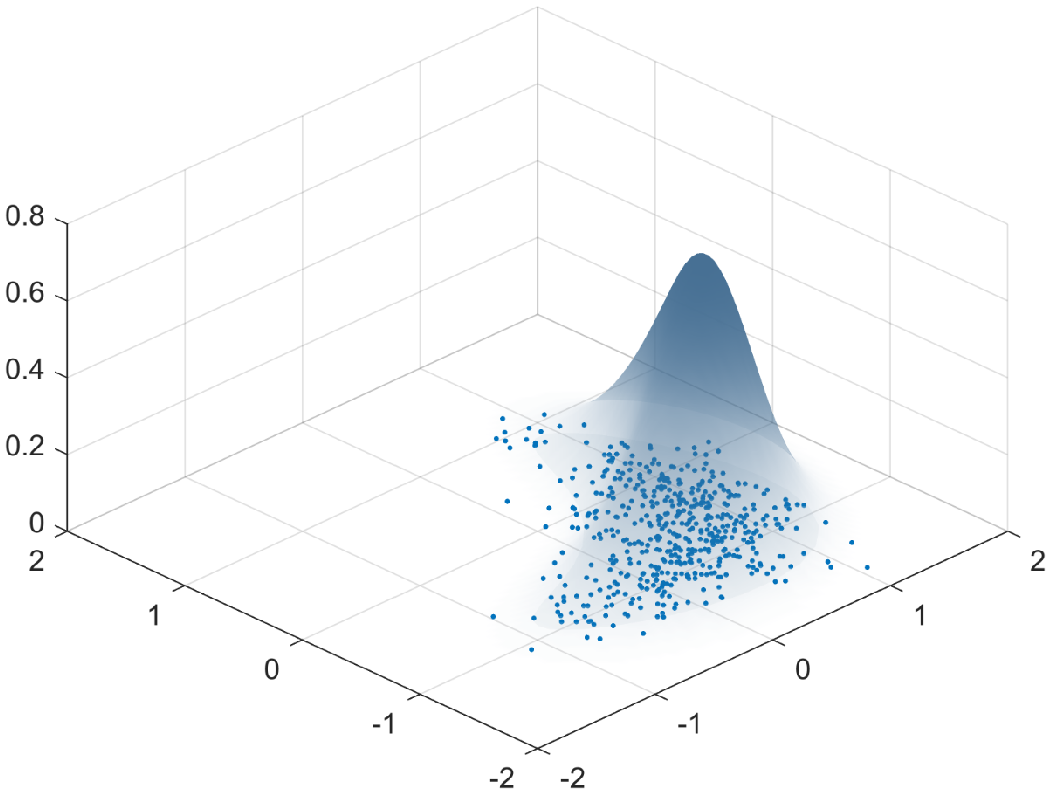
\includegraphics[width=1.5in]{./fig/fig2-a.pdf}
    }
    \subfloat[]{
        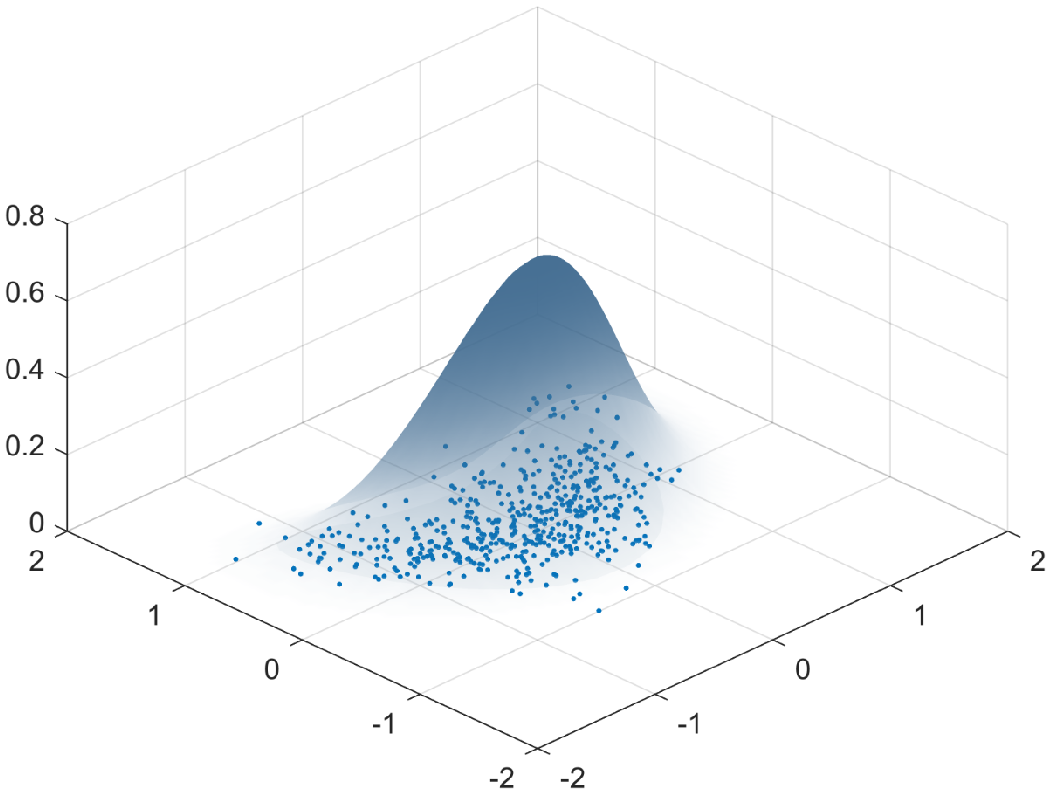
\includegraphics[width=1.5in]{./fig/fig2-b.pdf}
    }
    \quad
    \subfloat[]{
    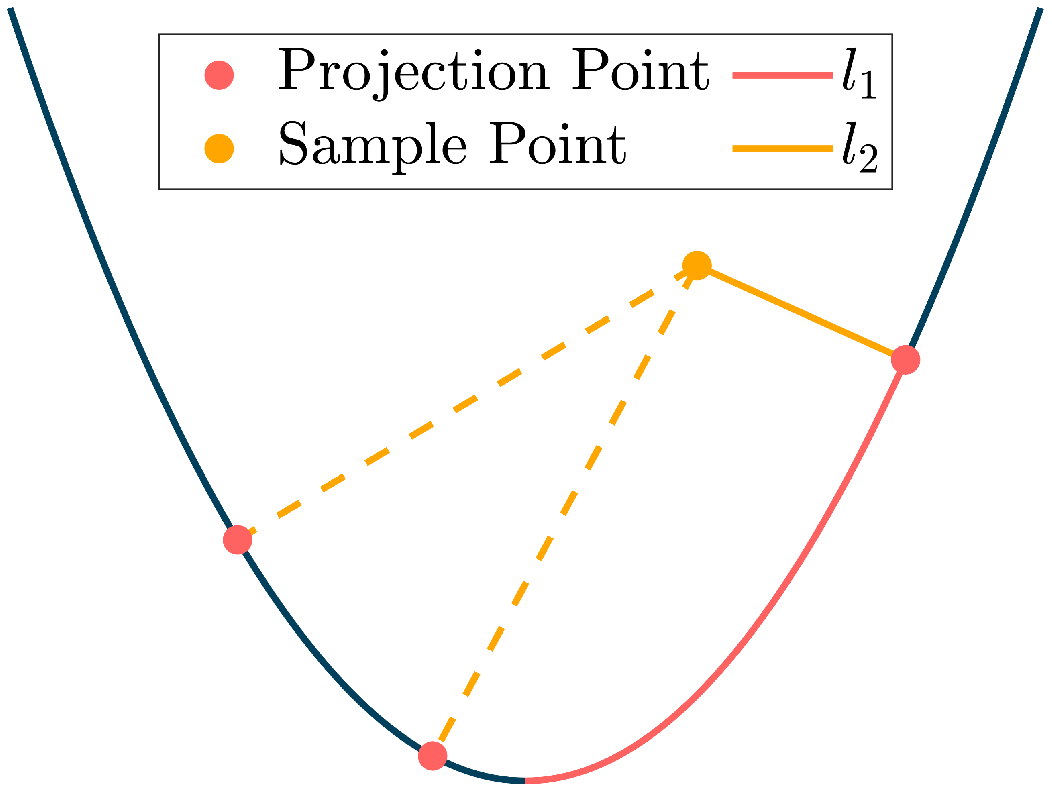
\includegraphics[width=1.5in]{./fig/fig2-c.pdf}
    }
    \subfloat[]{
        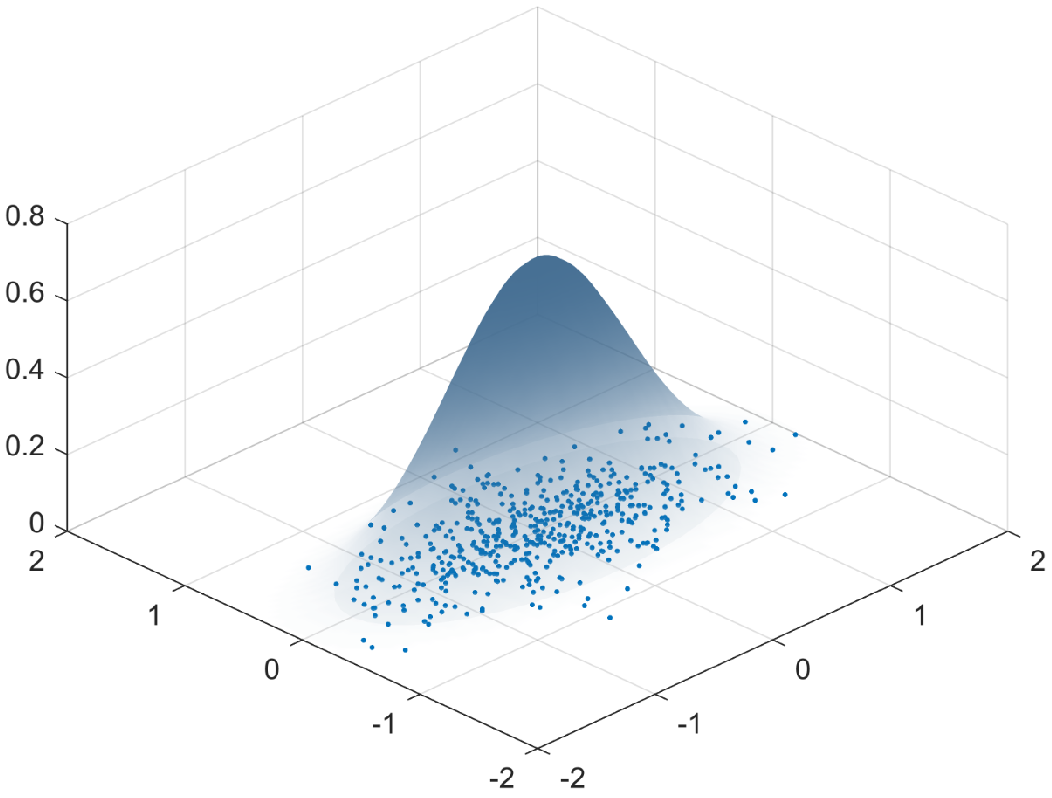
\includegraphics[width=1.5in]{./fig/fig2-d.pdf}
    }
    \caption{The data transformation process of FGMM.}
    \label{fig2}
\end{figure}

First, the k-means algorithm divides the dataset into $K$ classes. For each class of data, we transfer them to a new coordinate through PCA (Principal Component Analysis) :
\begin{equation}
    Y_i=Q_i \times (X_i-T_i)
\end{equation}
where $Q_i$ and $T_i$ denote the rotation matrix and translation vectors. $X_i$ is data which belongs to the $i^{th}$ components. The transformed data $Y_i$ presented in Fig.\ref{fig2}b have zero mean, and their principal axis aligns with the transformed x-axis. Noticed that we assume all data are two-dimensional in this paper.

The LSFM (least-squares fitting method) is used to fit the data using a parabolic curve. AcaGMM uses the projection point on the parabolic curve to replace the sample point for calculating the posterior probability. First, the distance between a sample point $\{x_{1t},x_{2t}\}$ and its projection point $\{z_{1},z_{2}\}$ satisfies:
\begin{equation}
    \begin{aligned}
        d^2 & =(z_{1}-x_{1n})^2+(z_{2}-x_{2n})^2 \\
        z_2 & =cz_1^2+b
    \end{aligned}
\end{equation}
the Lagrange method is used to find the closest projection point. The cubic function may have multiple solutions, which means a sample may have multiple projection points with the shortest distance. Then we calculate the arc length of the $j^{th}$ projection points $\{z_{1j},z_{2j}\}$:
\begin{equation}
    l_{1j}=\int_{(0,b)}^{(z_{1j},z_{2j})}\sqrt{(dz_{1j})^2+(dz_{2j})^2}
\end{equation}
eliminate $z_{2j}$, we have:
\begin{equation}
    l_{1j}=\frac{1}{2}z_{1j}\sqrt{4c^2z_{1j}^2+1}+\frac{1}{4|c|}ln(2|c|z_{1j}+\sqrt{4c^2z_{1j}^2+1})
\end{equation}
and the distance between $x_t$ and $z_j$ is:
\begin{equation}
    l_{2j}=\sqrt{(x_{1t}-z_{1j})^2+(x_{2t}-z_{2j})^2}
\end{equation}
where Fig\ref{fig2}.c illustrates the geometric meaning of $l_{1j}$ and $l_{2j}$.

Then we can calculate the probability of the sample $x_t$ via the sum of its projection points $z_j$:
\begin{equation}
    p_i(x_n|\theta_i)=\sum\limits^{J_t}_{j=1}\frac{exp(-l_{1j}^2/2\Sigma_1-l_{2j}^2/2\Sigma_2)}{2\pi\sqrt{|\Sigma_1\Sigma_2|}}
\end{equation}
where the parameter $\theta_i=(\mu_i,\Sigma_i,C_i,Q_i,T_i)$, and $J_t$ means the number of projection points of the sample $x_n$.

The EM algorithm is proposed for parameter estimation in AcaGMM. Due to the change in the probability density function, the parameter estimation method of AcaGMM differs from the conventional GMM. The procedure of the new EM algorithm is:

1) E-step: For each component, calculate the "expected" components of all samples:
\begin{equation}
    w_{in}=\frac{\alpha_ip_i(x_n|\theta_i)}{\sum^k_{s=1}\alpha_sp_s(x_n|\theta_s)}
    \label{eq1}
\end{equation}
where $w_{in}$ denotes $x_n$ posterior probability for the $i^{th}$ components.

2) M-step: For each component, calculate the maximum likelihood of the given sample. The weight of each component is then estimated from:
\begin{equation}
    \alpha_i=\frac{1}{N}\sum\limits^N_{n=1}w_{in}
\end{equation}

Then parameters $C_i,T_i,Q_i$ can be estimated from:
\begin{equation}
    (C^{new}_i,T^{new}_i,Q^{new}_i)=LSFM(PCA(X_i))
\end{equation}
where $X_i$ denotes samples belonging to the $i_{th}$ components, which can be classified by Eq. \ref{eq1}. $\mu_i$ can be estimated by the following method:
\begin{equation}
    \mu_i^{new}=\frac{\sum^N_{n=1}w_{in}x_n}{\sum^N_{n=1}w_{in}}+(Q_i^{new})^{\bf{T}}[0,b]^{\bf{T}}+T_i^{new}
\end{equation}
and $\Sigma_i$ can be estimated from:
\begin{equation}
    L_{sn}=\frac{\sum^{J_{in}}_{j=1}p(l^i_{sj}|0,\Sigma^{old}_{si})l^i_{sj}}{\sum^{J_{in}}_{j=1}p(l^i_{sj}|0,\Sigma^{old}_{si})}~(s=1,2)
\end{equation}
\begin{equation}
    \Sigma_{si}=\frac{\sum_{n=1}^Nw_{in}L_{sn}}{\sum_{n=1}^Nw_{in}}~(s=1,2)
\end{equation}
where $L_{1n}$ denotes the mean arc length of $x_n$'s projection points, and $L_{2n}$ means the average distance between $x_n$ and its projection points. It can be considered that samples $X_n$ undergoes a non-linear transformation to obtain $L_n=\{L_{1n},L_{2n}\}$, presented in Fig.\ref{fig2}d. $L_n$ satisfied the distribution of the conventional zero-mean Gaussian.

The above step represents a single iteration of the EM algorithm. Repeat the iteration and update the parameters until the relative difference of log-likelihood between two iterations is less than a preset threshold. FGMM introduces an FCMs (Fuzzy C-means) mechanism to accelerate the convergence speed of the EM algorithm.

\subsection{Dynamic Movement Primitive}
To enable the proposed method to adapt to writing tasks in different environments, the DMP is combined into the designed skill learning framework. The DMP is a LfD model based on dynamic systems\cite{Ijspeert2013}. It consists of a second-order dynamic system and a non-linear function, allowing it to encode motion trajectories with fewer parameters while maintaining stability. For the encoded trajectory, modifying the positions of the starting and ending points can also retain the original motion characteristics:
\begin{equation}
    \ddot y = \alpha(\beta(g-y)-\dot y) + f
    \label{eq4}
\end{equation}

To change the trajectory speed, a scaling term $\tau$ is added in front of the velocity variable $\dot y$:
\begin{equation}
    \tau^2 \ddot y = \alpha(\beta(g-y)-\tau \dot y) + f
\end{equation}

To decouple the non-linear equation from time, a canonical system $x(t)$ is used to drive the dynamic system:
\begin{equation}
    \tau \dot x = - \kappa x
\end{equation}

The first term in Eq.\ref{eq4} is a PD (Proportional-Derivative) system. To avoid overshooting and ensure stable convergence to the attractor, let the parameter $\beta = \alpha / 4$, rewriting the second-order dynamic system as a critically stable spring-damping system. The system ultimately converges stably to the position $g$. The second term $f$ in Eq.\ref{eq4} is a non-linear function that controls the intermediate process of convergence. The non-linear function $f$ can be expressed as:
\begin{equation}
    f(x)=\frac{\sum\limits_{i=1}^{N} \Psi_{i}(x) w_{i}}{\sum\limits_{i=1}^{N} \Psi_{i}(x)}x(t)(g-y)
    \label{eq5}
\end{equation}
where, $\Psi(t)$ is a Radial Basis Function (RBF), expressed as:
\begin{equation}
    \Psi_i(x)= \exp \left(-\frac{\left(x-\mu_i \right)^{2}}{2 \sigma_i^{2}}\right)
\end{equation}
where $N$ represents the number of RBF, $\mu_i$ represents the position of the $i^{th}$ basis function, and $\sigma_i$ represents the width of the $i^{th}$ basis function. $\omega_i$ represents the weight of the $i^{th}$ radial basis function, which needs to be obtained by learning from the demonstration trajectory. Given a demonstration trajectory, here we used the trajectory $y_{dms}=\mathcal{F}' _{gmr}(t)$ obtained by GMR, the expression for $f_{dms}$ can be derived from Eq.\ref{eq4}:
\begin{equation}
    f_{dms} = \tau^2 \ddot y_{dms} - \alpha(\beta (g-y_{dms})-\tau \dot y_{dms})
    \label{eq6}
\end{equation}
where Locally Weighted Regression (LWR) is used to determining the weight parameter $w_{i}$, which can control the $f(x)$ to fit $f_{dms}$.

\section{Methodology}
\subsection{System Description}
\begin{figure*}[!t]
    \centering
    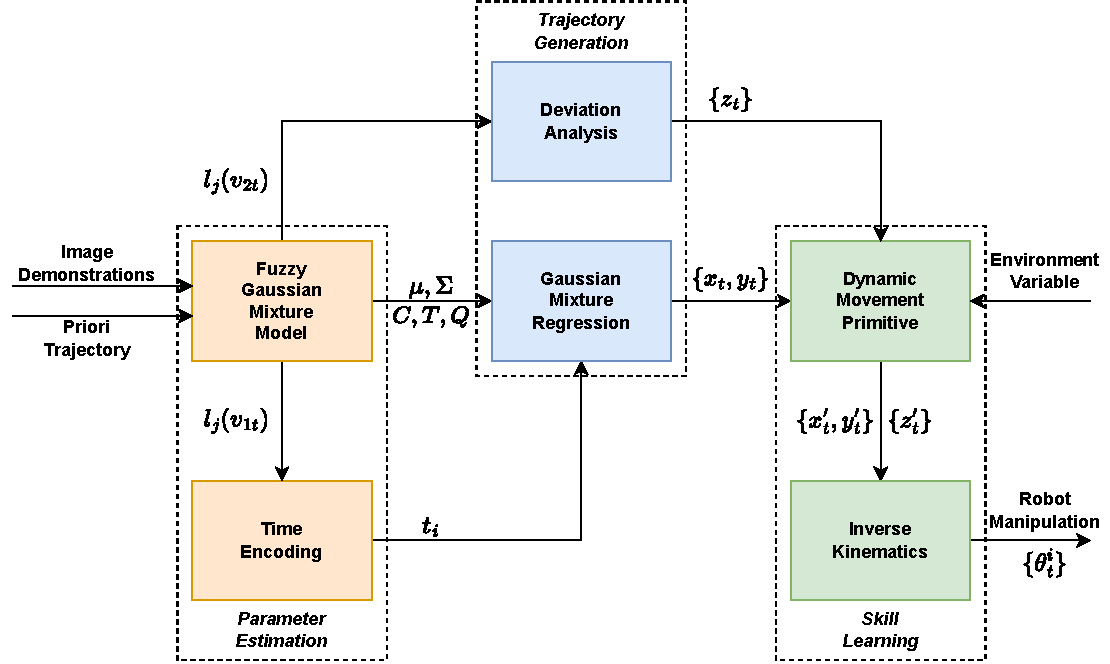
\includegraphics[width=6in]{./fig/fig1.pdf}
    \caption{Block diagram of the proposed system.}
    \label{fig1}
\end{figure*}
The block diagram presented in Fig. \ref{fig1} illustrates the framework of the imitation learning system for robotic handwriting tasks. The system can learn skills from static images and prior trajectories, particularly focusing on the deviation information within them, and ultimately achieving skill generalization in various environments. The entire system encompasses three aspects:

1)~Image Demonstration: The demonstration part transfers the writing skill to the robot through the character image written by a human. The proposed system enables robot learning parameters of FGMM from a static image. On the other hand, the priori information of time is attained by the priori trajectories, which explicitly show the implicit time information in the image.

2)~Skill Learning: With the parameters estimated in the previous part, we can encode the writing skill through GMR. The normal GMR method can generate the trajectory very well. However, the effect of learning the deviation among samples in the image is not that good. Therefore, we proposed a novel approach called deviation analysis to enhance the deviation learning ability of GMR.

3)~Motion Generalization: It is common to adjust the generalization effect of writing skills in different situations, like changing the size of the written font to adapt the various types of papers in the real world. DMP is used to make the skill have great generalization performance. DMP can encode not only the trajectory but also the end-effector orientation.



\subsection{Time Encoding}
Traditional vision-based demonstrations are mostly obtained by recording motion sequences to acquire demonstration trajectories. Data usually contains time sequences, and time-driven methods like GMR and DMP are used for motion encoding and skill learning. However, in some scenarios, the time sequence of demonstration trajectories is missing, like demonstrating writing skills through an image. A new method based on FGMM is proposed for encoding the time series of demonstration trajectories.
\begin{figure}[!t]
    \centering
    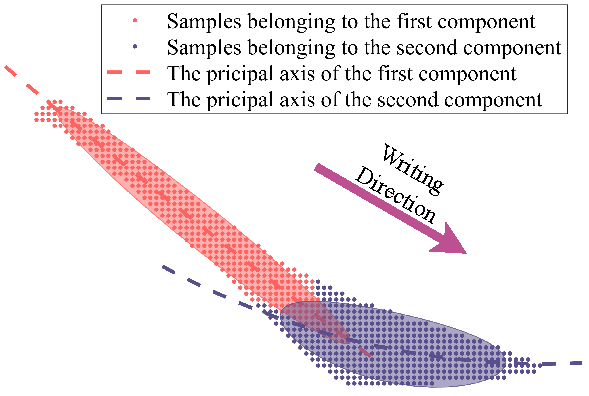
\includegraphics[width=3in]{./fig/fig3.pdf}
    \caption{Fitting Chinese stroke using FGMM.}
    \label{fig3}
\end{figure}

First, estimate the parameter of FGMM using the EM algorithm proposed before. Here we use a Chinese character stroke image as an example, presented in Fig.\ref{fig3}. The direction is needed to determine a general direction of movement. The direction does not need to be very precise. Most Chinese character strokes follow a sequence from left to right and from top to bottom, so the order of FGMM components can be determined. Each sample has a transformed point $L_n$ after a non-linear transformation during the parameter estimation. For most writing tasks involving movement along the principal axis, time information can be obtained through $L_{1n}$, which denotes the relative position of the sample on the principal axis. First we transfer the transformed sample from the first component $L_{1}^{(1)}=\{L_{11}^{(1)}, \hdots, L_{1n}^{(1)}\}$ to a zero starting point:
\begin{equation}
    t^{(1)}=\{L_{11}^{(1)}, \hdots, L_{1n}^{(1)}\}-min(L_{1}^{(1)})
\end{equation}

For the second component of transformed sample $L_{1}^{(2)}$, transfer them to the end of the first sequence:
\begin{equation}
    t^{(2)}=\{L_{11}^{(2)}, \hdots, L_{1n}^{(2)}\}-min(L_{1}^{(2)})+max(L_{1}^{(1)})
\end{equation}
if there are multiple components, repeat this process until the end. The time sequence is denoted as $\{t^{(1)},t^{(2)},\hdots,t^{(i)}\}$. Fig.\ref{fig4} presents the result of time encoding. The arrow on the sample point indicates the direction of time flow.
\begin{figure}[!t]
    \centering
    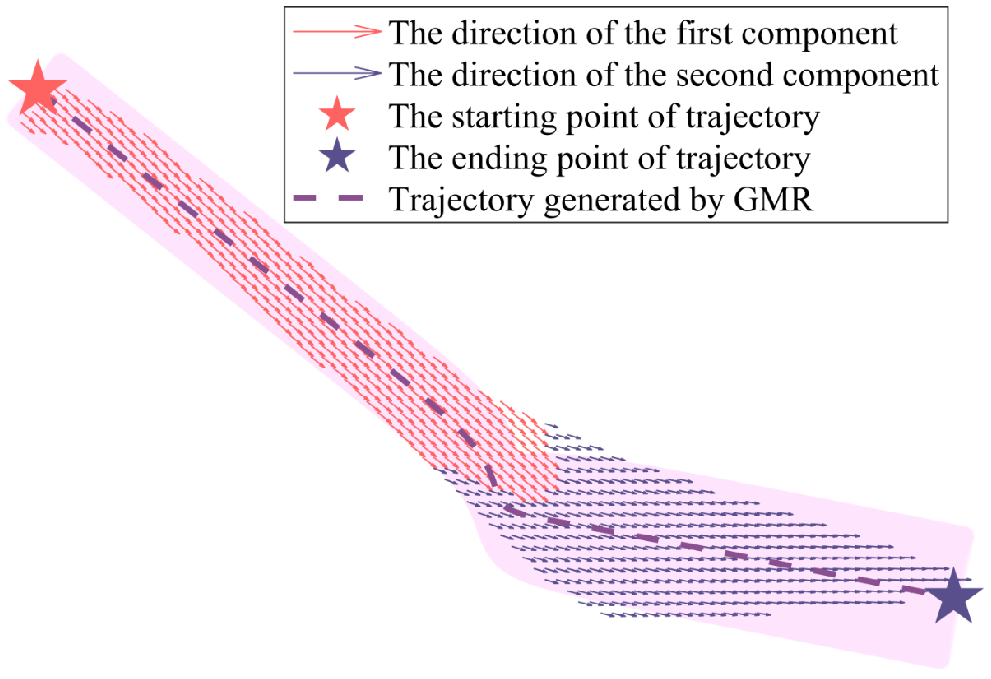
\includegraphics[width=3in]{./fig/fig4.pdf}
    \caption{The result of time encoding and GMR.}
    \label{fig4}
\end{figure}

After time encoding, the time-driven method can be used for motion planning in writing tasks. Gaussian Mixture Regression (GMR) is a statistical learning technique that combines the GMM with linear regression. GMR is used to address nonlinear regression problems by capturing the intrinsic structure of the data through a Gaussian mixture model, which is then used to perform regression analysis. GMR allows us to specify one dimension of the GMM as input, with the remaining dimensions as output. Here, the time sequence $t$ obtained before is used as the input, and the position $X=\{x_1,\hdots,x_n\}$ as the output to plan the writing trajectory. The regression function can be considered as obtaining the expectation of an event for the output $X$ conditional on the input $t$:
\begin{equation}
    \mathcal{F} _{gmr}(t)=E(X|t)
\end{equation}

Assume that $X$ and $t$ follow the Gaussian distribution, the event satisfies:
\begin{equation}
    X|t \sim G(\mu_X+\frac{\sigma_{21}}{\sigma_{1}}(t-\mu_t),\sigma_{2}-\frac{\sigma_{12}\sigma_{21}}{\sigma_{1}})
\end{equation}
where $\sigma_{1}$ and $\sigma_{2}$ denote the variance of $t$ and $X$, $\sigma_{12}$ and $\sigma_{21}$ denote the covariance between $t$ and $X$. Consider that the Gaussian mixture model can be seen as a linear combination of Gaussian distributions, the expectation can be written as:
\begin{equation}
    \mathcal{F} _{gmr}(t)=\sum\limits_{i=1}^{K}w_i(t)\eta_i(t)
\end{equation}
where
\begin{equation}
    w_i(t)=\frac{\alpha_{i}G(t|\mu_{i}(t),\sigma_{it})}{\sum_{i=1}^{K}\alpha_{i}G(t|\mu_{i}(t),\sigma_{it})}
\end{equation}
\begin{equation}
    \eta_i(t)=\mu_{iX}+\frac{\sigma_{21i}}{\sigma_{1i}}(t-\mu_{it})
    \label{eq2}
\end{equation}

In the previous part, the GMM is replaced with FGMM, which has better non-linear fitting capability. The regression function should be redesigned. Paper\cite{Yang2019c} proposes a new regression algorithm for FGMM. Notice that Eq.\ref{eq2} is a linear function, it defines the location of GMM's principal axis. For the FGMM, the corresponding axis can be obtained from the PCA inverse transformation:
\begin{equation}
    A_i'=Q_i^{\bf{T}}A_i+T_i
\end{equation}
where $A_i$ and $A_i'$ denote the original axis and transformed axis. The regression for FGMM can be denoted as:
\begin{equation}
    \mathcal{F}' _{gmr}(t)=\sum\limits_{i=1}^{K}w_i'(t)A_i'
\end{equation}
where the FGMM component should replace each Gaussian component in $w_i'$, the movement trajectory planning by GMR is presented in Fig.\ref{fig4}. Compared with Fig.\ref{fig3}, it can be seen that the trajectory highly overlaps with the principal axis.

\subsection{Deviation Analysis}
In some scenarios, such as transferring writing skills to robots, they need to learn not only the trajectory information of sample points but also the deviation among them. The pink area shown in Fig.\ref{fig4} denotes the covariance of trajectory generated by GMR. The fitting effect is not ideal. A new method based on FGMM is proposed. Analyse the deviation of samples to generate a variance sequence for a better fitting effect.

In addition to generating a trajectory from time input, GMR can also generate a corresponding covariance sequence $\{\Sigma_1,\hdots,\Sigma_t\}$. It denotes the covariance among samples in time $t$. The covariance matrix implicitly contains the posture and deviation of the trajectory. They can be obtained by eigenvalue decomposition:
\begin{equation}
    \Sigma_t=R_tD_tR_t^{-1}
\end{equation}
where $D_t$ and $R_t$ represent the eigenvalues and eigenvectors of the covariance matrix, respectively. According to the geometric meaning of eigenvalue decomposition, they also represent the scaling effect and rotation effect of the covariance matrix, respectively, which represent the deviation and posture information of the trajectory. $L_{2n}$ defines the distance between the transformed sample and the principal axis. It can be used to define a new scaling matrix. According to the $3\sigma$ rule, the new scaling matrix is defined as:
\begin{equation}
    D_t^{new}=\left[
        \begin{array}{cc}
            (\frac{1}{3}L_{2t})^2 & 0       \\
            0                     & D_{22t}
        \end{array}
        \right]
    \label{eq3}
\end{equation}
the new covariance sequence is:
\begin{equation}
    \Sigma^{new}_t=R_tD^{new}_tR_t^{-1}
\end{equation}



\section{Experiments}
\subsection{Simulation}
In this part, The proposed method is verified through simulation. A Chinese calligraphy image is used as the demonstration image, denoted in Fig.\ref{fig5}. Paper \cite{Li2022} propose an observation based algorithm which can extract strokes from the Chinese character image. As shown in Fig.\ref{fig5}(a), the Chinese character is divided into four strokes. Each stroke contains temporal information, which can be used to indicate the writing direction and the order of seven components, as Fig.\ref{fig5}(b) and (c) denotes. Fig.\ref{fig5}(b) and (c) also show the result of fitting the Chinese character image by conventional GMM and FGMM, respectively. The conventional GMM need to use 8 components to fit the character well. In contrast, the FGMM only requires 7 components.
\begin{figure*}[!t]
    \centering
    \subfloat[]{
        
\includegraphics[width=2in]{./fig/fig5-a.pdf}
    }
    \subfloat[]{
        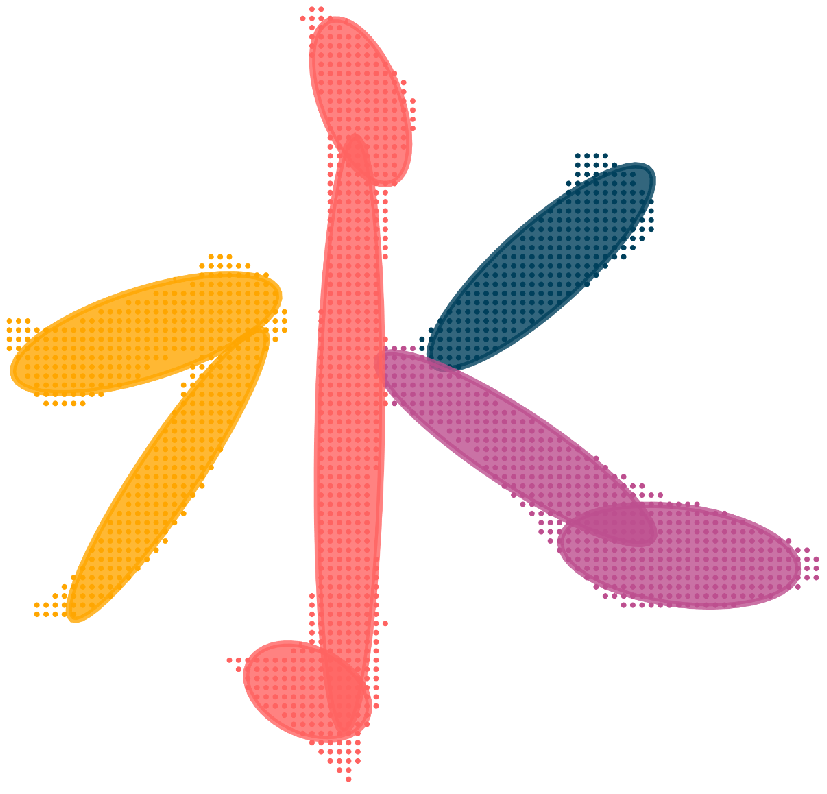
\includegraphics[width=2in]{./fig/fig5-b.pdf}
    }
    \subfloat[]{
        
\includegraphics[width=2in]{./fig/fig5-c.pdf}
    }
    \quad
    \subfloat[]{
        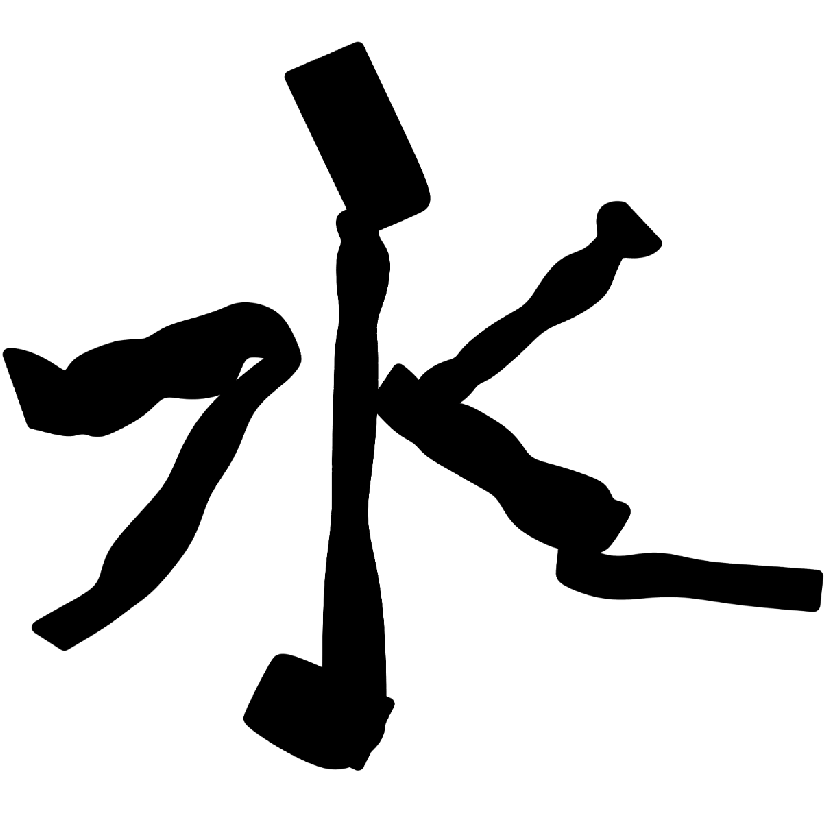
\includegraphics[width=2in]{./fig/fig5-d.pdf}
    }
    \subfloat[]{
        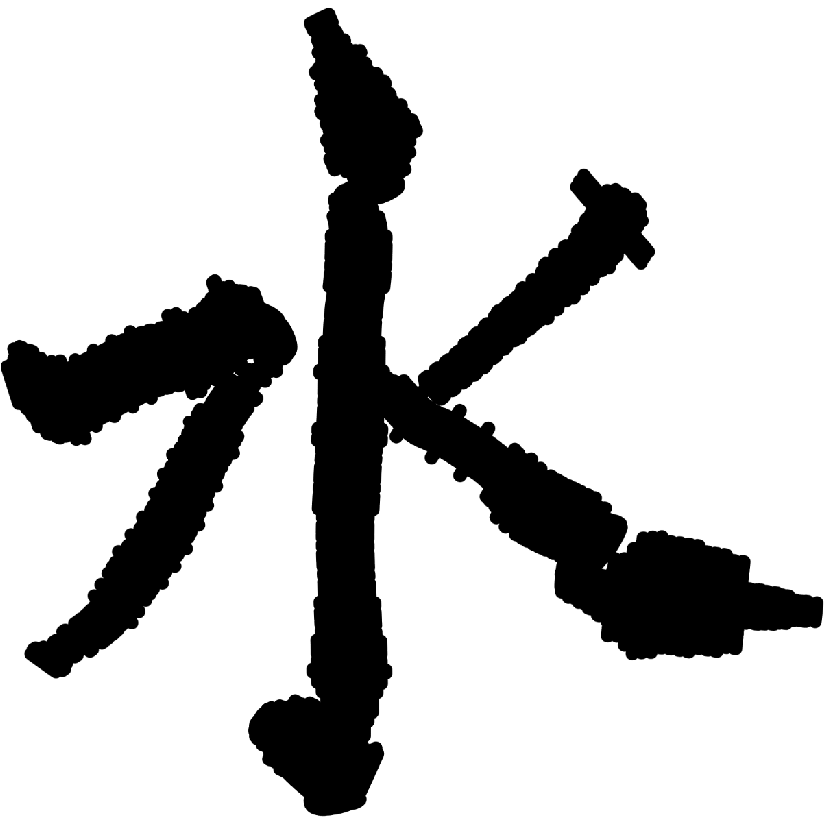
\includegraphics[width=2in]{./fig/fig5-e.pdf}
    }
    \subfloat[]{
        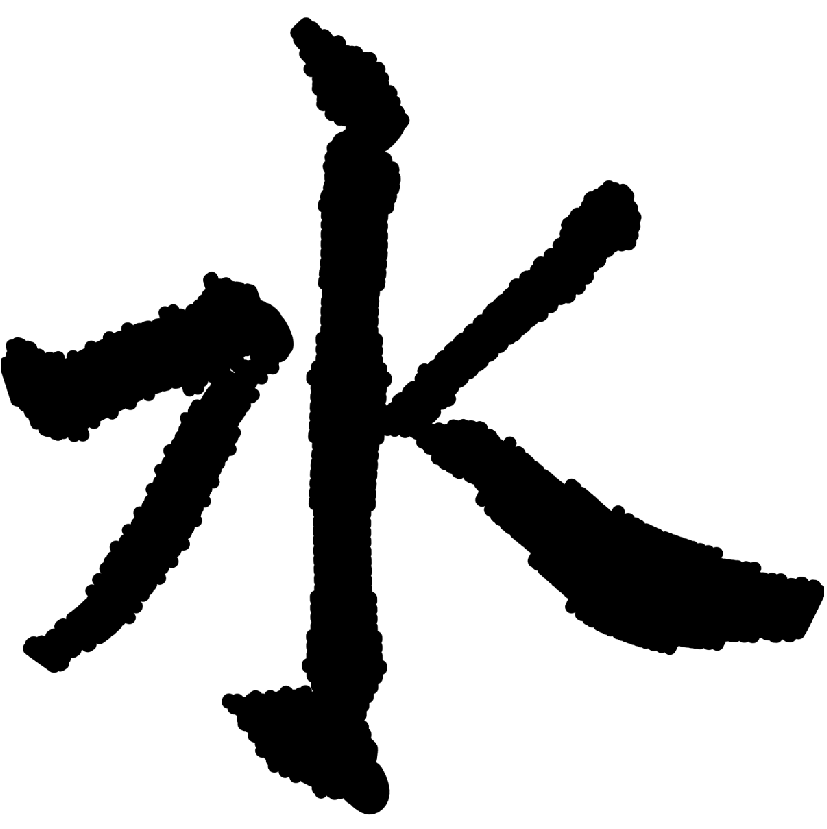
\includegraphics[width=2in]{./fig/fig5-f.pdf}
    }
    \caption{The writing simulation of Chinese character "water".}
    \label{fig5}
\end{figure*}

The sample points are time-encoded for each stroke based on the known writing direction and component order. The new GMR method and DA is used to learn the character's writing trajectory and deviation degree. In the simulation part we need to simulate the effect of robot writing on the computer. The following three methods will be compared to the effect of writing tasks: the GMM without DA, the GMM with DA and the FGMM with DA. To maintain the accuracy of the comparison, the writing tasks are simulated based on a unified method. Assume the discrete trajectory is $\{(x_1,y_1),\hdots,(x_N,y_N)\}$, and the covariance matrix sequence is $\{\Sigma_1,\hdots,\Sigma_N\}$. At time t, the writing trajectory is defined as:
\begin{equation}
    o_t =[cos(p),sin(p)]\sqrt{3\Sigma_t}+[x_t,y_t]~~(-\pi<p<\pi)
\end{equation}
where the area represented by $o_t$ indicates the writing trace at time t. The writing simulation results for the three methods are denoted in Fig.\ref{fig5}. 

To compare the fitting effect of the simulation results with the demonstration image, we introduce 10 commonly used Image Quality Assessment (IQA) methods as evaluation metrics, denoted in Table.\ref{tab1}. They are all Full Reference (FR) methods, which can evaluate the differences between the simulation results and the demonstration image. The evaluation results are presented in Table.\ref{tab2}. The DA improve the fitting effect of Chinese character a lot. The improvements in FGMM further enhance the fitting effect.  
\begin{table}[!t]
\centering  
\caption{IQA METRICS AND MEANINGS}
\label{tab1}
\begin{tabularx}{3in}{lX}
\toprule
Metric & Description\\
\midrule
PSNR & Peak signal-to-noise ratio. A higher score indicates a higher similarity.\\
FSIM & Feature Similarity Index. A higher score indicates a higher similarity.\\
SSIM & Structural Similarity Index. A higher score indicates a higher similarity.\\
VSI & Visual Saliency-based Index. A higher score indicates a higher similarity.\\
VIF & Visual Information Fidelity. A higher score indicates a higher similarity.\\ 
IFC & Image Fidelity Criterion. A higher score indicates a higher similarity.\\
DISTS & Differential Stimulation Similarity. A lower score indicates a higher similarity.\\
MSE & Mean Square Error. A lower score indicates a higher similarity.\\
VOI & Variation of Information. A lower score indicates a higher similarity.\\
LPIPS & Learned Perceptual Image Patch Similarity. A lower score indicates a higher similarity.\\
\bottomrule
\end{tabularx}
\end{table}

% \begin{table*}[!t]
% \centering  
% \caption{IQA METRICS AND MEANINGS}
% \label{tab2}
% \begin{tabular}{ccccccccccc}
% \toprule
% Model & PSNR$\uparrow$ & FSIM$\uparrow$ & SSIM$\uparrow$ & VSI$\uparrow$ & VIF$\uparrow$ & IFC$\uparrow$ & DISTS$\downarrow$ & MSE$\downarrow$ & VOI$\downarrow$ & LPIPS$\downarrow$\\
% \midrule
% GMM & 10.7447 & 0.7896 & 0.7867 & 0.7665 & 0.0203 & 0.0452 & 0.3535 & 5477.8718 & 2.9374 & 0.3354 \\
% GMM+DA & 11.5709 & 0.7901 & 0.7928 & 0.8018 & 0.0225 & 0.0493 & 0.3522 & 4528.9159 & 2.8622 & 0.3058 \\
% \textbf{FGMM+DA} & \textbf{12.1143} & \textbf{0.7990} & \textbf{0.8019} & \textbf{0.8126} & \textbf{0.0236} & \textbf{0.0514} & \textbf{0.3463} & \textbf{3996.2290} & \textbf{2.8019} & \textbf{0.2951} \\
% \bottomrule
% \end{tabular}
% \end{table*}

\begin{table}[!t]
    \centering  
    \caption{THE IQA RESULT OF THE SIMULATION}
    \label{tab2}
    \begin{tabular}{cccc}
    \toprule
    Metric & GMM & GMM+DA & \textbf{FGMM+DA} \\
    \midrule
    PSNR$\uparrow$ & 10.7447 & 11.5709 & \textbf{12.1143} \\
    FSIM$\uparrow$ & 0.7896 & 0.7901 & \textbf{0.7990} \\
    SSIM$\uparrow$ & 0.7867 & 0.7928 & \textbf{0.8019} \\
    VSI$\uparrow$ & 0.7665 & 0.8018 & \textbf{0.8126} \\
    VIF$\uparrow$ & 0.0203 & 0.0225 & \textbf{0.0236} \\
    IFC$\uparrow$ & 0.0452 & 0.0493 & \textbf{0.0514} \\
    VOI$\downarrow$ & 2.9374 & 2.8622 & \textbf{2.8019} \\
    MSE$\downarrow$ & 5477.8718 & 4528.9159 & \textbf{3996.2290} \\
    DISTS$\downarrow$ & 0.3535 & 0.3522 & \textbf{0.3463} \\
    LPIPS$\downarrow$ & 0.3354 & 0.3058 & \textbf{0.2951} \\
    \bottomrule
    \end{tabular}
\end{table}

\subsection{Generalization Verification}
In this part we will verify the generalization performance of the method. In the real world, the writing skills should be able to reproduce correspondingly in a variety of scenarios, like writing in different sizes of paper. Here the same Chinese character is used as an example to verify the performance of the writing skills reproduction.

Assuming the paper size for reproducing the writing skills is half the size of the demonstration image, the starting and ending points of the Chinese character strokes need to be re-determined. Here, the one-point perspective is used to determine the new starting and ending points. Then the proposed framework can reproduce the writing skills to fit this new scenario. Fig.\ref{fig6} denotes the demonstrative samples after time encoding and the reproduction of writing skills in $X$ and $Y$ dimension. The reproduction trajectories and their starting and ending points are represented in Fig.\ref{fig7}.

\begin{figure*}[!t]
    \centering
    \subfloat[]{
        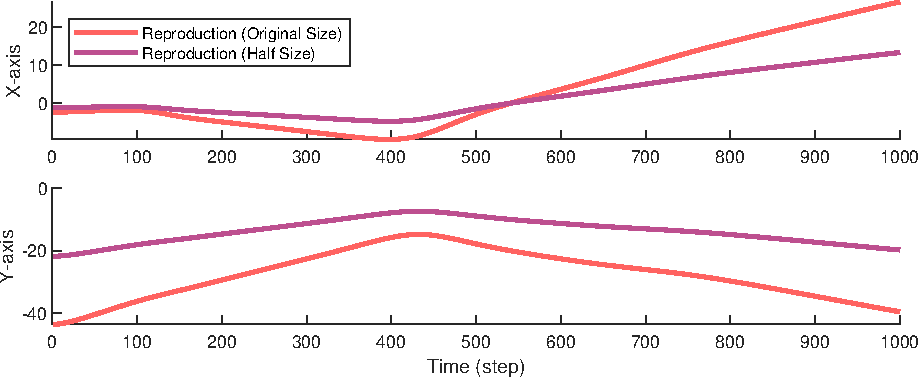
\includegraphics[width=3in]{./fig/fig6a.pdf}
    }
    \subfloat[]{
        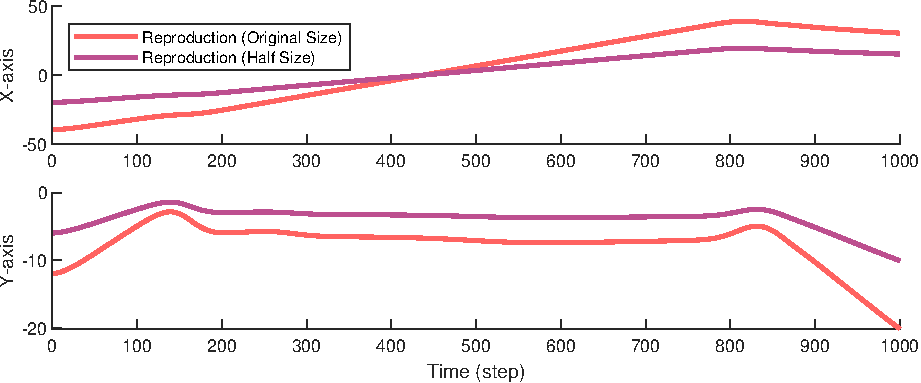
\includegraphics[width=3in]{./fig/fig6b.pdf}
    }
    \quad
    \subfloat[]{
        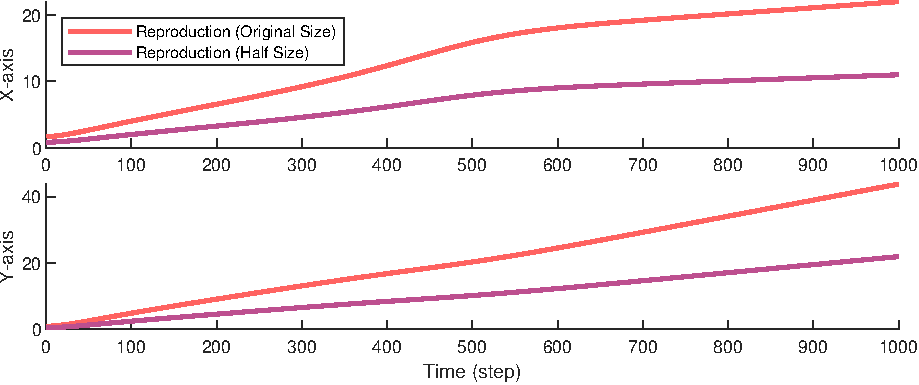
\includegraphics[width=3in]{./fig/fig6c.pdf}
    }
    \subfloat[]{
        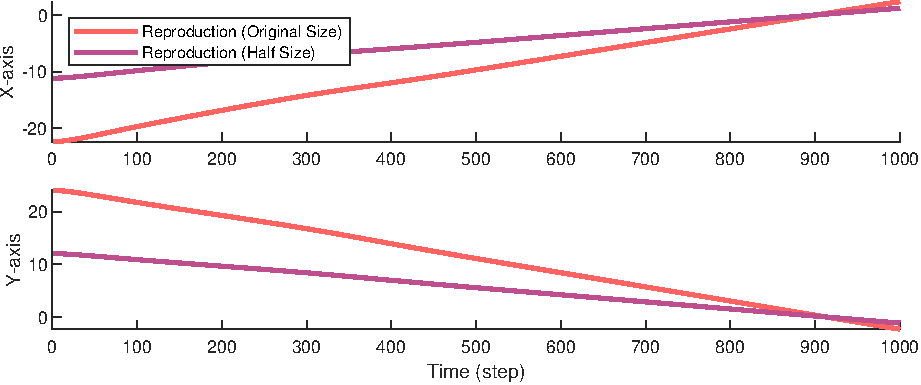
\includegraphics[width=3in]{./fig/fig6d.pdf}
    }
    \caption{The reproduction of writing skill for each stroke.}
    \label{fig6}
\end{figure*}

\begin{figure}[!t]
    \centering
    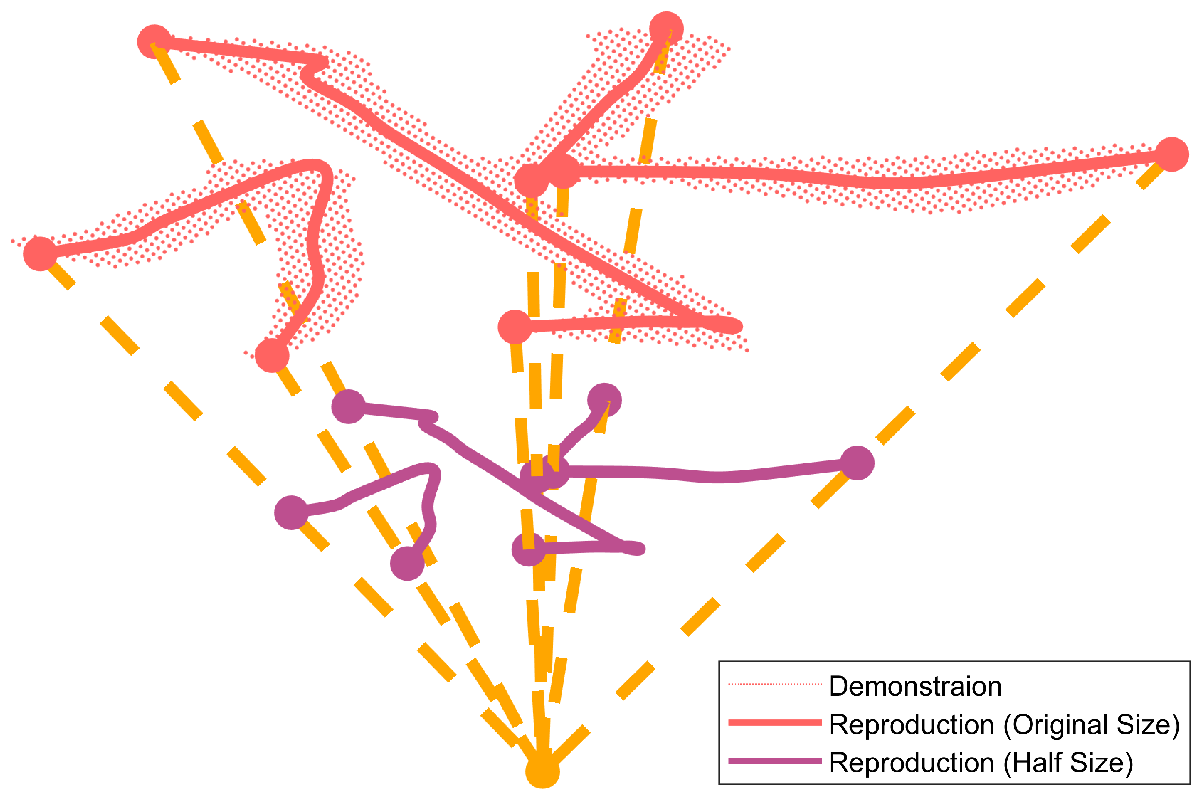
\includegraphics[width=3in]{./fig/fig7.pdf}
    \caption{The new starting and ending points for each stroke determined by one-point perspective. And the reproduction of writing skill for the whole Chinese character.}
    \label{fig7}
\end{figure}

\subsection{Real-World Experiment}
In this part, we conducted real-world experiment to validate the effectiveness of the proposed method on the platform represented in Fig.\ref{fig8}.a. The Elite EC66 robot, which is designed to mimic the human arm's anatomy, has six DoF, enabling it to perform a wide range of motion. A webcam is used to capture the demonstration image. To validate the efficacy of DA, we employed the traditional Chinese writing instrument, the brush pen, as the end-effector. This writing instrument controls the thickness of the strokes by varying the height of it. Compared to fountain pens, the brush pen exhibits a higher sensitivity in controlling the stroke thickness. However, due to its minimal stiffness, most of force sensors are unable to obtain effective force information during the writing process. Therefore, the implementation of a vision-based control approach is adopted for the robot, in lieu of force control. The height of the bursh pen is described by a quadratic function of the thickness of its stroke above the writing surface\cite{Guo2022}, indicating a non-linear relationship that can be mathematically expressed as:
\begin{equation}
    H_t=-k(D_{t11}^{new})^2+H_0
\end{equation}
where $k$ is a positve constants, which is determined by the parameter of the brush pen. $D_{t11}^{new}$ denotes the thickness of strokes calculated by Eq.\ref{eq3}. $H_t$ represents the height of the brush pen above the writing surface in time $t$, which $H_0$ is a constant indicates the initial height. Here the parameter $k$ and $H_0$ are designated as 0.2 and 240, respectively. The writing trajectories are represented in Fig.\ref{fig8}.b, and the real-world experience is represented from Fig.\ref{fig8}.c to Fig.\ref{fig8}.f.
\begin{figure*}[!t]
    \centering
    \subfloat[]{
        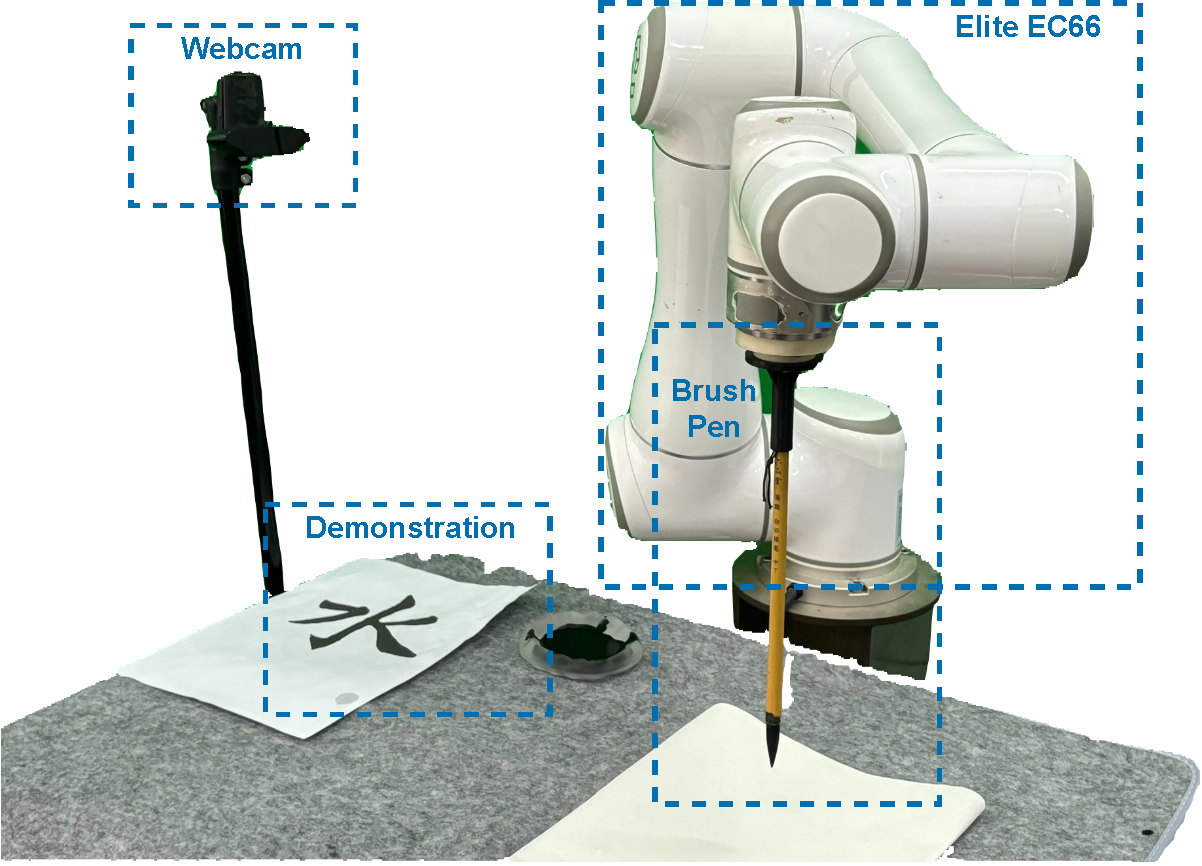
\includegraphics[width=3in]{./fig/fig8a.pdf}
    }
    \subfloat[]{
        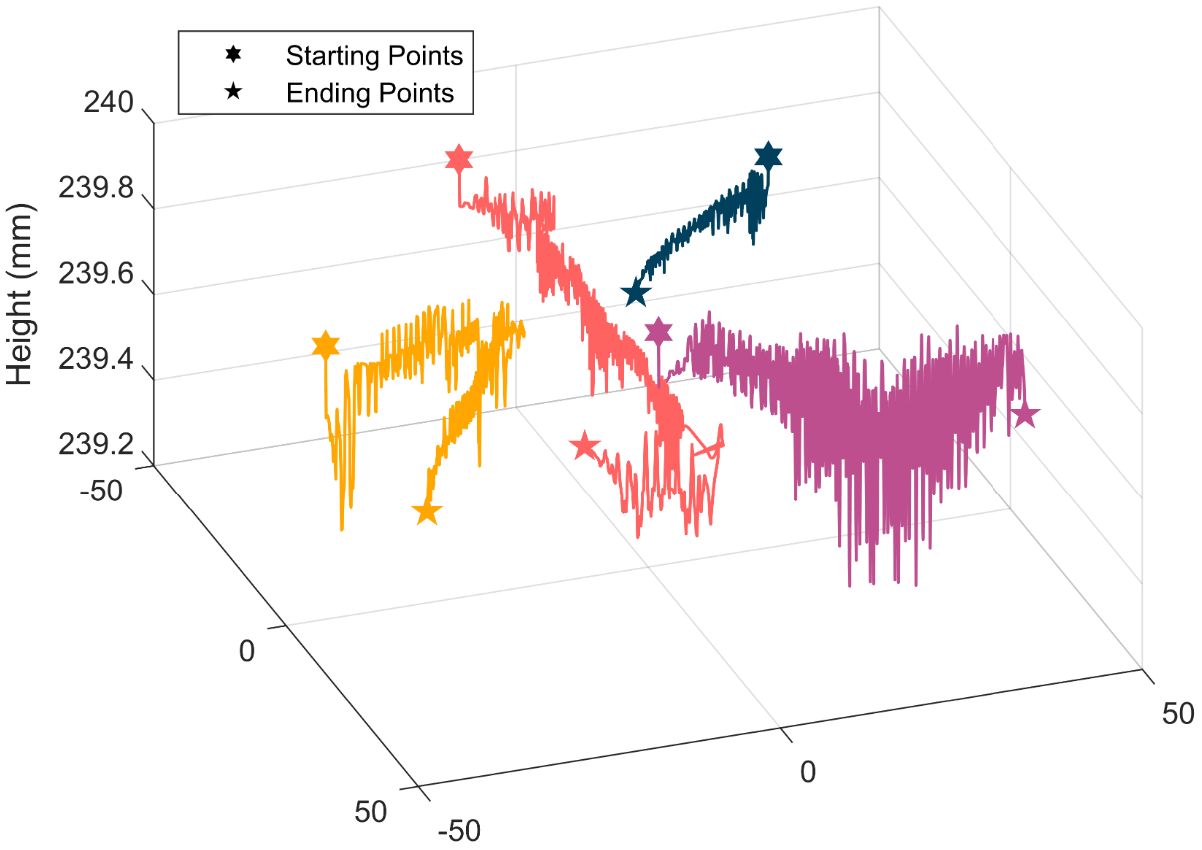
\includegraphics[width=3in]{./fig/fig8b.pdf}
    }
    \quad
    \subfloat[]{
        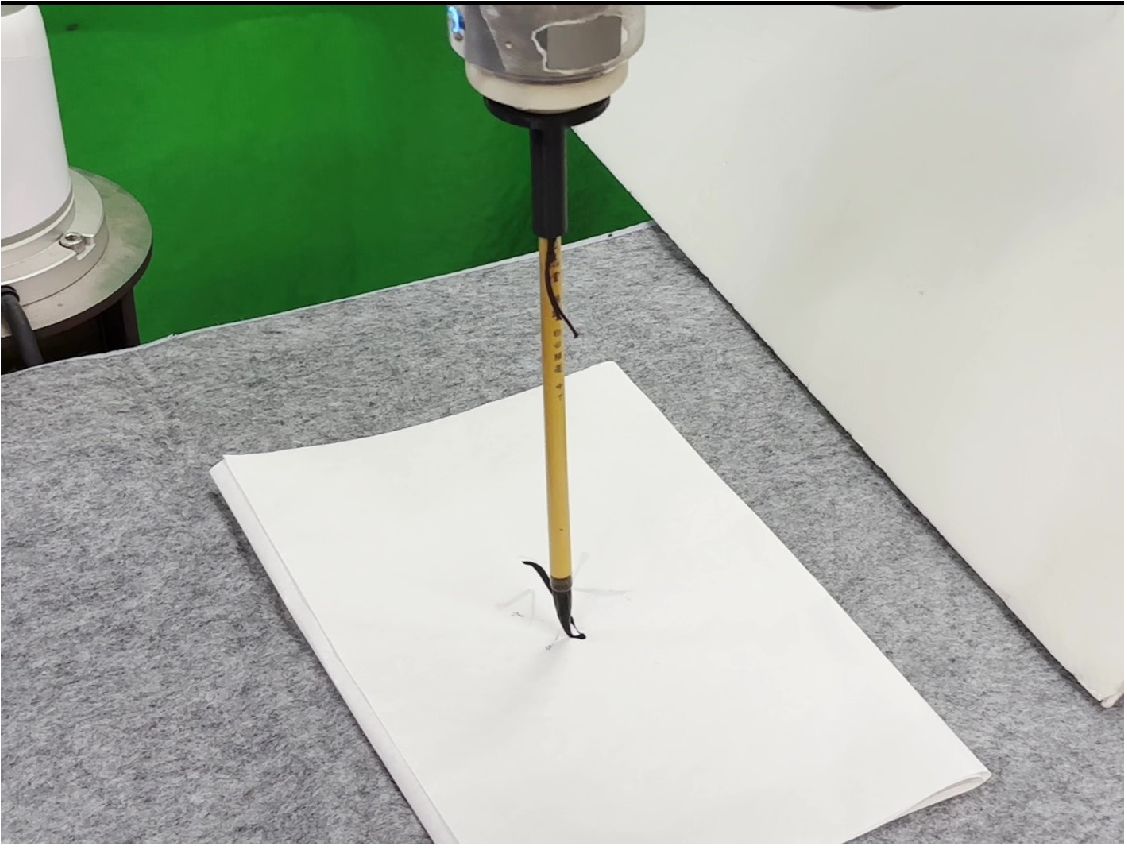
\includegraphics[width=1.5in]{./fig/fig8c.pdf}
    }
    \subfloat[]{
        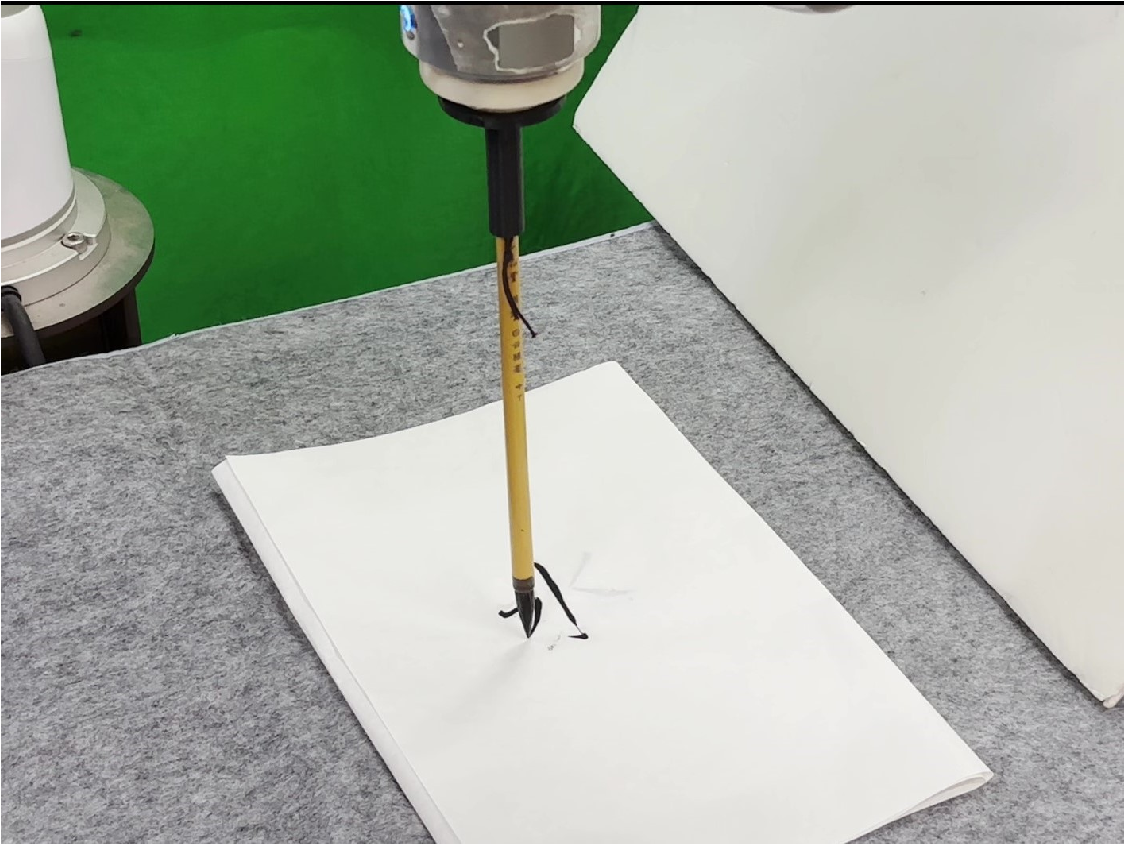
\includegraphics[width=1.5in]{./fig/fig8d.pdf}
    }
    \subfloat[]{
        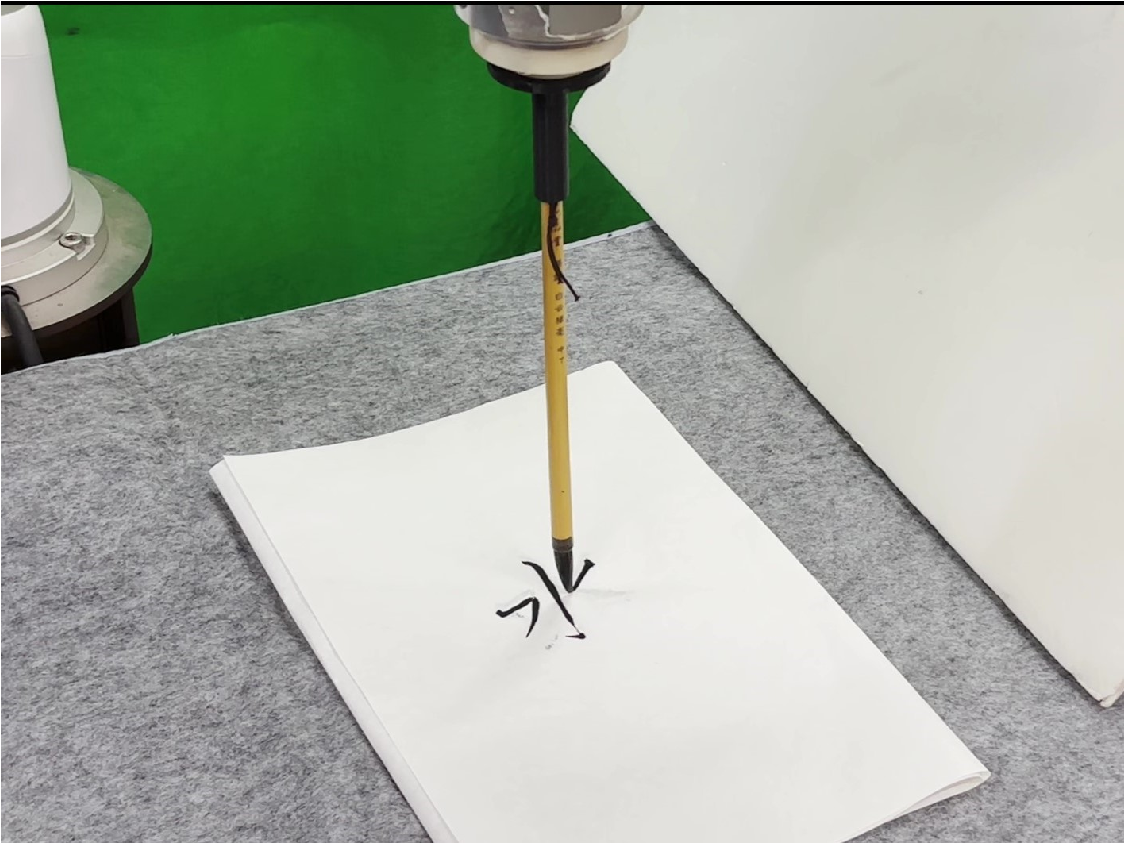
\includegraphics[width=1.5in]{./fig/fig8e.pdf}
    }
    \subfloat[]{
        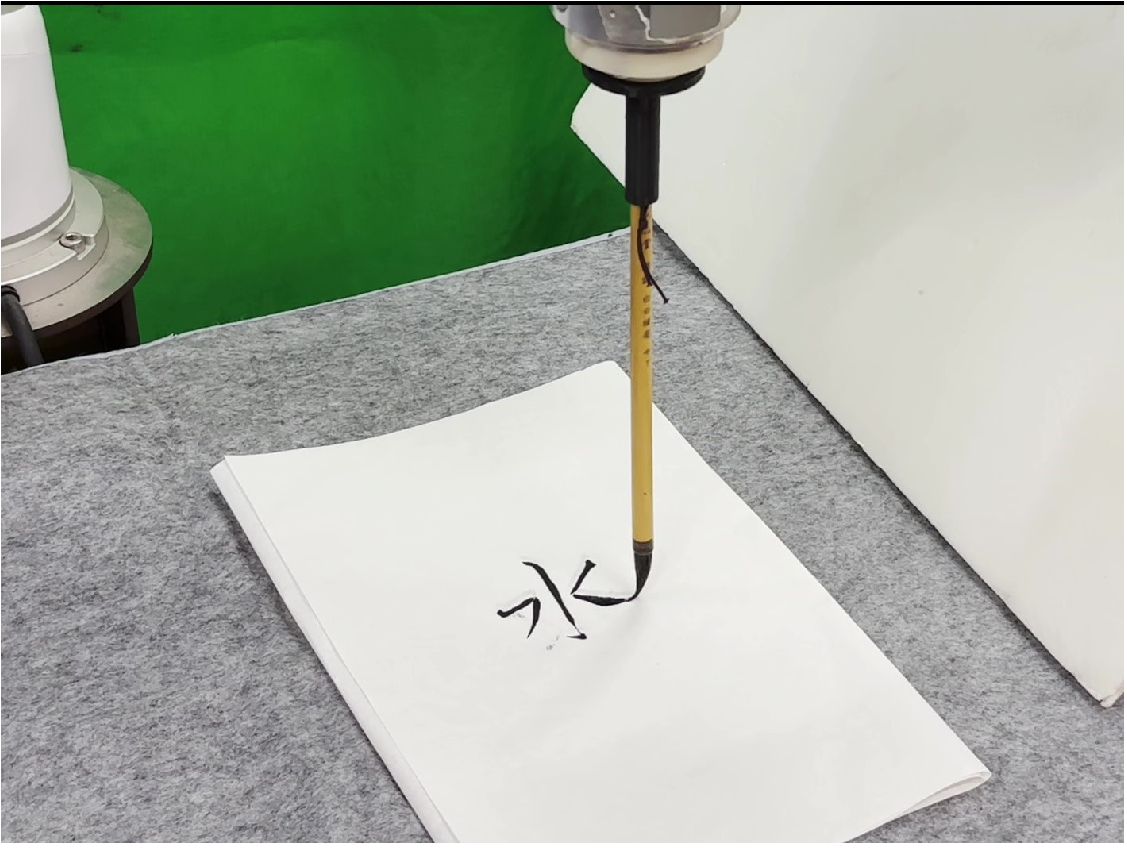
\includegraphics[width=1.5in]{./fig/fig8f.pdf}
    }
    \caption{The reproduction of writing skill for each stroke.}
    \label{fig8}
\end{figure*}

Then the performance of generalization is verified. Giving different sizes of square-grid paper, the robot can adaptively change the reproduction of writing skill, as Fig.\ref{fig9} presents.
\begin{figure}[!t]
    \centering
    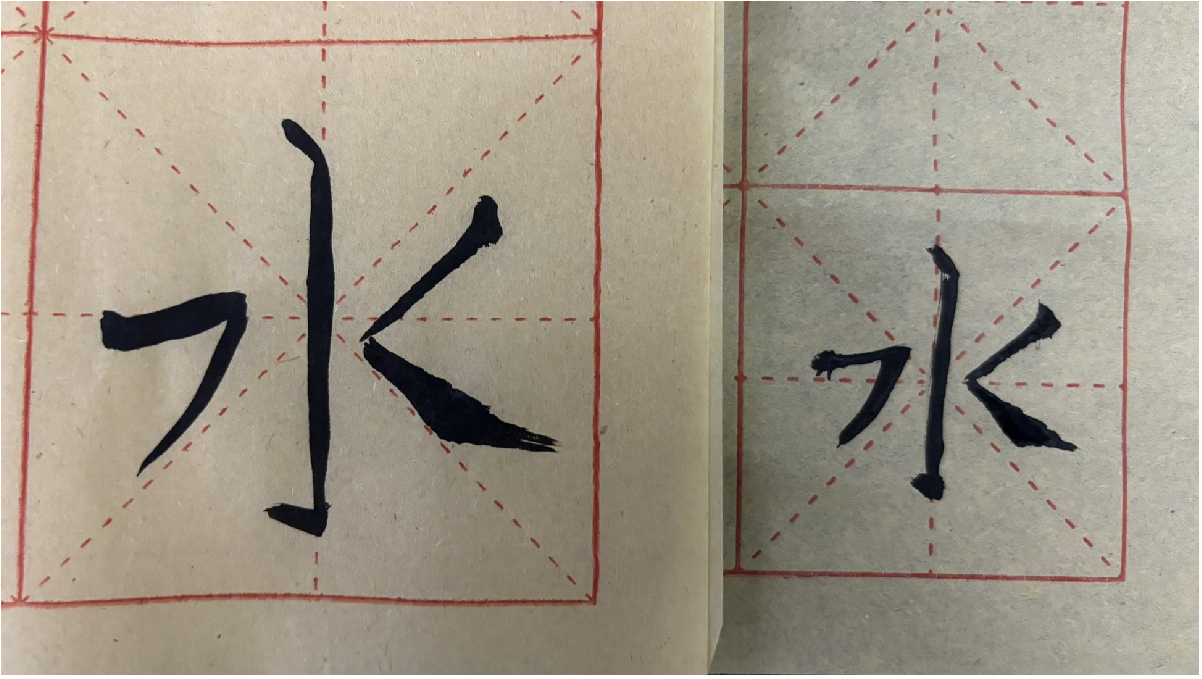
\includegraphics[width=3in]{./fig/fig9.pdf}
    \caption{The reproduction}
    \label{fig9}
\end{figure}

\section{Conclusion}






\bibliographystyle{IEEEtran}
\bibliography{IEEEabrv,reference.bib}
\end{document}
